	% -----------------------------------------------
% Styl pro psaní diplomových a bakalářských prací
% Určeno pro překlad pdfcsLaTeXem
% -----------------------------------------------
\documentclass[a4paper,12pt]{book} % pro oboustranný tisk zvolte {book}!
% velikost stránky
\usepackage[tmargin=2cm,bmargin=2.5cm,rmargin=2cm,lmargin=3.5cm]{geometry}
% volba kódování, nastaveno je unicode
\usepackage[utf8]{inputenc}
% \usepackage[cp1250]{inputenc}
% \usepackage[latin2]{inputenc}
\usepackage[english]{babel}
%\def\refname{Literatura}
% pomocná makra pro sazbu matematických výrazů
\usepackage{amssymb} %na psaní dvojitých písem a zvlastních znaků (např. \varkappa)
\usepackage{amsmath}
% balíček pro vkládání obrázků
\usepackage{graphicx}
% balíček pro obrázky na krajích stránky 
%\usepackage{floatflt}
% balíček pro křížové odkazy
\usepackage[unicode,bookmarksopen,colorlinks=false,plainpages=false,urlcolor=blue,pdfpagelabels]{hyperref}
% balíček pro vkládání hypertextových odkazů
\usepackage{url}

\usepackage{float}


\usepackage[numbers]{natbib}

% -----------------------------------------------
% Přepínač mezi bakalářskou a diplomovou prací, 
% barevným a černobílým logem a mezi studentem a studentkou (vypracoval/vypracovala apod.)
% -----------------------------------------------
\newif\ifbakal\bakaltrue
\newif\ifbarva\barvafalse
\newif\ifstudentka\studentkafalse

% -----------------------------------------------
% Údaje o práci – doplní se i do bibliografické identifikace, pouze v prohlášení je nutné vložit jméno vedoucího práce, které není v 1. pádě
% -----------------------------------------------
\newcommand{\nazevcz}{Kalibrace a monitorování astročásticových teleskopů}
\newcommand{\nazev}{Calibration and monitoring of astroparticle telescopes}
\newcommand{\student}{Daniel Staník}
\ifbakal%
  \newcommand{\program}{B0533A110007  Applied Physics}%
  \newcommand{\obor}{1702R001  Applied Physics  (AFYZ)}%
  %\else%
  %\newcommand{\program}{N1701 Fyzika}%
  %\newcommand{\obor}{7504T055 Učitelství fyziky pro střední školy}%
\fi
\newcommand{\rokod}{2022}
\newcommand{\vedouci}{Ing. Ladislav Chytka, Ph.D.}
\newcommand{\abstrakt}{%
Lorem ipsum dolor sit amet, consectetur adipiscing elit. Curabitur et lectus sit amet lectus vestibulum dignissim. Cras sit amet enim vitae mi elementum blandit eget nec tortor. Curabitur eget eros vitae arcu luctus varius commodo vel mauris. Nam elementum convallis pretium. Nunc dignissim pulvinar urna, nec blandit ante fringilla at. Ut et magna purus, vel pellentesque massa. In tortor nisi, faucibus condimentum cursus ut, sollicitudin quis leo. Ut at purus nec arcu accumsan tincidunt id id massa. Nam id vehicula mi.}
% -----------------------------------------------
\newcommand{\abstrakten}{%
Lorem ipsum dolor sit amet, consectetur adipiscing elit. Curabitur et lectus sit amet lectus vestibulum dignissim. Cras sit amet enim vitae mi elementum blandit eget nec tortor. Curabitur eget eros vitae arcu luctus varius commodo vel mauris. Nam elementum convallis pretium. Nunc dignissim pulvinar urna, nec blandit ante fringilla at. Ut et magna purus, vel pellentesque massa. In tortor nisi, faucibus condimentum cursus ut, sollicitudin quis leo. Ut at purus nec arcu accumsan tincidunt id id massa. Nam id vehicula mi.}
% klíčová slova
\newcommand{\klic}{klíčové slovo 1, klíčové slovo 2, \ldots}
\newcommand{\klicen}{keyword 1, keyword 2, \ldots}
\newcommand{\pocetstran}{xx}
\newcommand{\pocetpriloh}{x}

% -----------------------------------------------
% Definice vlastních maker pro usnadnění psaní
% a opakování symbolů při zlomu řádku
% -----------------------------------------------
% implikace se opakuje
\def\Plyne{\Rightarrow\discretionary{}{\hbox{$\Rightarrow$}}{}}
% -----------------------------------------------
% ekvivalence se opakuje
\def\Ekviv{\Leftrightarrow\discretionary{}{\hbox{$\Leftrightarrow$}}{}}
% -----------------------------------------------
% % plus '+' se opakuje při zalomení řádku
\mathchardef\plus="202B
\mathcode`\+="8000
{\catcode`\+=\active
\gdef+{\plus\nobreak\discretionary{}{\hbox{$\plus$}}{}}}
% opakování - při zalomení řádku
\newsavebox{\minusbox}
\savebox{\minusbox}{\hbox{$-$}}
\def\aktivniminus #1{{\catcode`#1=13 \bgroup \uccode`~=`#1
\uppercase{\egroup\gdef~}{\mathminus\discretionary{}{\copy\minusbox}{}}}}
% % -----------------------------------------------
% % rovnitko '=' se opakuje
\def\aktivnirovnitko #1{{\catcode`#1=13 \bgroup \uccode`~=`#1
\uppercase{\egroup\gdef~}{\mathequal\discretionary{}{=}{}}}}
% -----------------------------------------------
% zrušení mezery za čárkou v matematickém reľimu
\mathcode`,="002C

% -----------------------------------------------
% Úprava matematické sazby
% -----------------------------------------------
\def\sgn{\mathop{\rm sgn}\nolimits}
\def\tg{\mathop{\rm tg}\nolimits}
\def\cotg{\mathop{\rm cotg}\nolimits}
\def\arctg{\mathop{\rm arctg}\nolimits}
% -----------------------------------------------
% vektory polotučným skloněným písmem
\DeclareFontFamily{OT1}{bssbf}{}
\DeclareFontShape{OT1}{bssbf}{m}{n}{<5> <6> <7> <8> <9> <10> <11> <12> <14.4> <17> <20> <20.74> <25> bssb10}{}
\newcommand{\vek}{\fontencoding{OT1}\fontfamily{bssbf}\selectfont}
\renewcommand{\vec}[1]{\hbox{\vek #1}\hspace*{1.5pt}}
% polotučná řecká písmena
\def\bgomega{\vec{\char151}}
     \def\bgOmega{\vec{\char10}}
     \def\bggamma{\vec{\char130}}
     \def\bgvarphi{\vec{\char161}}
     \def\bgphi{\vec{\char148}}
     \def\bgxi{\vec{\char142}}
     \def\bgtau{\vec{\char146}}
     \def\bgeta{\vec{\char134}}
     \def\bgmu{\vec{\char139}}
     \def\bgnu{\vec{\char140}}
     \def\bvarrho{\vec{\char157}}
     \def\bgsigma{\vec{\char145}}
     \def\bgpsi{\vec{\char150}}
     \def\bgchi{\vec{\char149}}
     \def\bgvartheta{\vec{\char154}}
%\renewcommand{\thefigure}{\arabic{figure}}
%\renewcommand{\theeuqation}{\arabic{euqation}}

\raggedbottom %přidaný kvůli špatnýmu řádkování
% ---------------------------------------------------------------
% Samotná práce
% ---------------------------------------------------------------
\begin{document}
% -----------------------------------------------
% Titulní strana
% -----------------------------------------------
\pagestyle{empty}
\setbox0=\hbox{\LARGE\scshape Joint Laboratory of Optics}
\centerline{\LARGE\scshape  Palacký University Olomouc}

\bigskip
\centerline{\LARGE\scshape Faculty of Science}
   
\bigskip
\centerline{\box0}
  
\vfill
\centerline{\LARGE\bfseries \ifbakal{BACHELOR}\else{DIPLOMOVÁ}\fi\ THESIS}

\bigskip
\begin{center}
{\huge\nazev}  


\vfill
\ifbarva\includegraphics[height=3cm]{up_logo_color}\else%
\includegraphics[height=3cm]{up_logo_bw}\fi

\vfill

\noindent%
\begin{tabular}{ll}
Author\ifstudentka{a}\fi: & {\bfseries\student}\\
Study program: &\program\\
Field of study: &\obor\\
Form of study:& Full-time\\
Supervisor:& \vedouci\\
Deadline:& April~\rokod
\end{tabular}
\end{center}

% ---------------------------------------------------------------
% Prohlášení
% -----------------------------------------------
\newpage
\hbox{~}

\vfill

\begin{center}
{\bf DECLARATION}
\end{center}

\noindent
I hereby declare that I elaborated this bachelor thesis independently under the supervision 
of  Ing. Ladislav Chytka, Ph.D.,  using  only  information  sources  referred  in  the  Literature chapter. \\
{}\vspace{3ex}

\noindent
In~Olomouc~\today   \hfill\parbox[t]{6cm}{\centering\null\dotfill\\\student}

% -----------------------------------------------
% Bibliografická anotace
% -----------------------------------------------
\newpage
\input{bibl_identifikace}

%%%% Tady začínáme %%%%%%%%%%%%%%%%%%%%%%%%%%%%%%%%%%%%%%%%%%%%%%%%%%%%%%%%%%
\newpage
%%%%%%%%%%%%%%%%%%%%%%%%%%%%%%%%%%%%%%%%%%%%%%%%%%%%%%%%%%%%%%%%%%%%%%%%%%%%%
\widowpenalty =10000
\pagestyle{plain}
\let\cleardoublepage\clearpage %odstanění dvojitých stran
% -----------------------------------------------
% Obsah je generován automaticky, změny se projeví po 2 překladech
% -----------------------------------------------
\tableofcontents

% -----------------------------------------------
% Úvod
% -----------------------------------------------
\chapter*{Introduction}
\addcontentsline{toc}{chapter}{Introduction}

Lorem ipsum dolor sit amet, consectetur adipiscing elit. Curabitur et lectus sit amet lectus vestibulum dignissim. Cras sit amet enim vitae mi elementum blandit eget nec tortor. Curabitur eget eros vitae arcu luctus varius commodo vel mauris. Nam elementum convallis pretium. Nunc dignissim pulvinar urna, nec blandit ante fringilla at. Ut et magna purus, vel pellentesque massa. In tortor nisi, faucibus condimentum cursus ut, sollicitudin quis leo. Ut at purus nec arcu accumsan tincidunt id id massa. Nam id vehicula mi. 

\url{http://exfyz.upol.cz/didaktika/}

% -----------------------------------------------
% Kapitoly lze ukládat do zvláštních souborů...
% -----------------------------------------------
% -----------------------------------------------
% Vlastní text práce (kapitoly práce)
% -----------------------------------------------

% -----------------------------------------------
\chapter{Astroparticle detection}
% -----------------------------------------------
More than 100 years have passed since Victor Franz Hess first encontered cosmic radiation. Since those times the techniques and methods of detection have been strongly improved. We have moved up from elevating electroscopes by ballons to observe growing electric charge to specialized techniques, which allows us to measure particles' energies, trajectories, etc.

% -----------------------------------------------
\section{Cosmic rays and particles}
% -----------------------------------------------
Cosmic rays is a term for radiation and energetic particles striking earth atmosphere with an origin in a space sources (neutron stars, supernovas, black holes, etc). We divide them into two major groups - primary and secondary. Primary cosmic rays are the original cosmic particles, which strike the Earth's athmosphere. Secondary cosmic rays (also refered as showers) are particles, which have origin in particle interaction between primary cosmic rays and the athmosphere.
\par
\subsection{Primary cosmic rays}
Primary cosmic rays consist of protons ($95 \%$), helium nuclei ($4 \%$), electrons and other heavy nuclei (up to iron). However, only the energetic rays make their way to the athmosphere. The Earth's magnetic field affects their trajectories and prevents the low-energetic (less than 100 MeV) particles from arriving to the athmosphere \cite{Kliewer}. 
\par
Part of primary cosmic rays are also Ultra-high energy cosmic rays (UHECRs), which we refer in the next chapter.
\par 
Neutrinos are also a part of cosmic radiation, but their interaction with matter is very rare, so they are very hard to detect. The special underwater detectors are developed to detect some of them. 
\subsection{Secondary cosmic rays}
Secondary cosmic rays are created by interaction of high-energetic particles of primary component with air's nucleis, such as nitrogen. They consist of low-energetic and high-energetic muons, gamma photons, electrons and positrons. Most of muons travel up to the earth's surface although their half-life is only about 2.2 microseconds before they decay into electrons. Due to their high relativistic speeds, their half-life is increased for external observers. 




% -----------------------------------------------
\section{Ultra-high energy cosmic rays (UHECRs)}
UHECRs are particles with energies from $10^{18}$ to $10^{20}$ eV, which is much more than particles created on Cern's Large hadron colider (LHC) with energies about $10^{13}$. Due to their high energies, the trajectory remains nearly unchanged by space magnetic fields \cite{Benjamin_Skuse}.
\par
UHECRs' origin is yet unknown, but it is supposed and experimentally proved that they come from outside of the Milky Way. Some theoretical physicists expects, that the one possible source of UHECRs acceleration are the starburst galaxies. One of the UHECR possible candidate is proton. 
\par
In many particle physics experiments, some form of calorimeter is used to determine the particles' energy and direction. In case of UHECRs, the air molecules of athmosphere have the function of calorimeter.
When the UHECR interacts with athmospheric nuclei, the cascade of particles is induced. This cascade concists of three main components: electromagnetic, hadronic and muonic. It is also refered as extensive air shower (EAS).
\par
In case of ultra-high energy proton striking an air molecule, kaons, baryons, nuclear fragments and mostly pions are created. Together, they are refered as hadronic component. The pions with short lifetime decay into electromagnetic sub-shower. The behaviour of pions with longer lifetime is energy-dependent. At higher energies they reinteract with atmospheric nuclei and feed hadronic and electromagnetic component. At lower energies they decay into muonic component with muonic neutrinos. The muons with short lifetime decay into electrons and positrons with neutrinos, which joins the electromagnetic cascade, while the others reach the Earth's surface carrying the energy, which we are unable to detect. The UHECR's cascade scheme could be seen on picture \ref{cascade}. 
\begin{figure}[H]
 \centering
 \includegraphics{up_logo_bw}
 \caption{UHECR's cascade, taken from nevimco \ref{nevimco}.}
 \label{cascade}
 
\end{figure}

\par

The electromagnetic cascade consisting of electron, positrons, gama photons carries the most of UHECR's original energy. With increasing depth, the cascade develops by decaying the photons into electron and positron pairs, which again emit photons and this process repeats. The cascade develops until the the energy treshold is reached, where the ionization is higher than the radiation losses. \ref{Tomankova2016_1000061954}.


\par
One of the main parameters of electromagnetic cascade is $X_{max}$ - the point along the shower axis, where is the maximum of deposited energy.

% -----------------------------------------------
\section{UHECRs detection techniques}
Nowadays there are three main proven techniques to detect UHERCs - 
air fluorescence, surface particle detection and Cherenkov light detection.

\subsection{Air fluorescence}
The electrons and positrons from electromagnetic cascade excite nitrogen molecules, which then deexcite and emit fluorescence light in UV spectre with two main wavelengths 337 and 357 nm. The intensity of this light is directly proportional to the calorimetric energy of the shower.
\par
However, the intensity of this light is very low, and thus the measurements must be done in dark nights with no light smog. Even a low intensity of external sources could led to detection of false events or worse - the unwanted light could damage the very sensitive equipment. 
\par
The detection equipment are mostly the superreflective UV mirrors which focus part of the UV shower into the PMT or into the camera based on PMTs. It it necessary to have atmospheric monitoring system (temperature, humidity, pressure etc.) along with the detection part, because the fluorescence is highly dependent on these conditions.  
\par
The main advantage of fluorescence detection is the fact, that by measuring and integrating the light profile we are able to calculate the total calorimetric energy. However, corrections   

\par
The FAST telescope, on which we focus in this thesis, is considered to be a fluorescence telescope.
\subsection{Surface particle detection}
Surface particle detection is a method, which is based on detecting individual particles from EAS. There are two proven surface techniques to detect EAS - by scintillators or water Cherenkov detectors. To detect the EAS full geometric distribution, the huge surface needs to be covered by surface detectors. 


\par
Compared to fluorescence detection method, the surface detectors don't require the dark night and any light exposure is not a threat for them.  



\subsection{Cherenkov light detection}


\subsection{Hybrid detection}

\section{UHECRs observatories}
\subsection{Pierre Auger observatory}
% -----------------------------------------------

\subsection{Telescope array project}
% -----------------------------------------------
% %%%%%%%%%%%%%%%%%%%%%%%% End of file %%%%%%%%%%%%%%%%%%%%%%%%

% -----------------------------------------------
% -----------------------------------------------
% Vlastní text práce (kapitoly práce)
% -----------------------------------------------

% -----------------------------------------------
\chapter{FAST telescope}
% -----------------------------------------------
The  Fluorescence  detector  Array  of  Single-pixel  Telescopes  (FAST) is an international project of fluorescence telescope sensitive to UHERCs. 
\par
Until today there are four prototypes in active service. Three of them are situated in Black Rock Mesa site of the Telescope Array experiment in central Utah and one in Argentina near Pierre Auger Observatory.
\par
The main goal of FAST project is to develop a cheap fluorescence telescope, which could be used in future to cover the wide surface area. This new oncoming fluorescence telescope array should be able  
to fully reconstruct the geometry of UHERCs induced UV shover by combining the information from telescopes, which has encountered some event at the same time. 
% -----------------------------------------------
\section{Principle of operation}
% -----------------------------------------------
Main detection part of telescope consists of superreflective UV mirrors and photomultipliers. 


\par
The entire telescope along with monitoring systems and other instruments is situated in a hut with remote shutter, where it is protected from negative metrological phenomena, such as rain or fast wind, but also from dust and aerosols. Exposure of mirrors to any of this phenomena could lead to reduction of theirs reflectivity. It is also neccessary to monitor and protect PMTs from unwanted light sources. Even a low-intensity sources could decrease PMT's service life.
% -----------------------------------------------

\section{Remote control and monitoring}
% -----------------------------------------------

%------------------------------------------------

\section{}
% -----------------------------------------------



% -----------------------------------------------
% %%%%%%%%%%%%%%%%%%%%%%%% End of file %%%%%%%%%%%%%%%%%%%%%%%%

% -----------------------------------------------
% -----------------------------------------------
% Vlastní text práce (kapitoly práce)
% -----------------------------------------------

% -----------------------------------------------
\chapter{Instrumentalization and measurement preparation}
% -----------------------------------------------
To perform all of neccesary measurements we need to use various types of optical and electronical equipment.
% -----------------------------------------------
\section{Integration sphere}
% -----------------------------------------------
The Integration sphere (IS) is a special optical equipment, which can be used either as 
% -----------------------------------------------

\section{Photomultiplier}
% -----------------------------------------------

%------------------------------------------------

\section{Silicon PM}
% -----------------------------------------------

%------------------------------------------------

\section{Hardware for experiment and measurement control}
% -----------------------------------------------
\subsection{Raspberry Pi}

\subsection{STM32 based microcontrolers}
% -----------------------------------------------
% %%%%%%%%%%%%%%%%%%%%%%%% End of file %%%%%%%%%%%%%%%%%%%%%%%%

% -----------------------------------------------
% -----------------------------------------------
% Vlastní text práce (kapitoly práce)
% -----------------------------------------------

% -----------------------------------------------
\chapter{Calibration UV optical source}
% -----------------------------------------------
Blah blah we need it.
% -----------------------------------------------
\section{Karlsruhe UV source}
% -----------------------------------------------


 \begin{figure}[H]
 \centering
 \includegraphics[scale=0.09, angle = 270, origin = c]{./pictures/KarlsRuhe}
 \caption{UV source conctructed according to KIT's template.}
 \label{UVsource}
\end{figure}


Our main task was to test this UV source's longtime stability and develop possible fixes and upgrades.

% -----------------------------------------------

\section{Testing and measurement of UV source}
% -----------------------------------------------
For calibration UV source, the longtime stability of optical power and pulse geometry is very important. Because there were no specialized apparatus for this measurement, we had to built and program one by ourselves.
\subsection{Measuring apparatus}
For measuring the optical power we use PM16 power meter (PM) and for determining the pulse geometry we use XP2262 PMT with signal output connected to 2-channel PicoScope 2205A MSO usb osciloscope. XP2262 PMT is held on $U \approx -680$ V by HV voltage source.
\par
We also use DS18B20 thermometer for PMT temperature monitoring and keysight 34461a multimeter for checking voltages.

\par
The PMT, power meter and the optical head of UV source are mounted in the IS's ports. The IS stops the unwanted external light and distributes the optical power to PMT and power meter. 
\par
The entire apparatus is driven by Raspberry Pi (RPi). The RPi takes care of data acquisiton and could be used to set the parameters of the UV source. It could be easilly accessed over internet for data download or for user to control the experiment.
\par
Osciloscope was programmed in C language according to its programmer's manual \ref{PicoScope}. It is capable of 2ns sampling which is enough to capture rising edges of the pulses. The RPi sets basic parameters (DC coupling, range etc.) and then activates osciloscope's trigger (rising edge). After sampling, RPi receives all samples from osciloscope's memory.

\par
Main component (IS,PW, PMT with HV source, UV source) are situated in protection box to prevent unwanted manipulations and touching the HV parts.The apparatus could be seen on fig. \ref{aparature1} and \ref{aparature2}.

\begin{figure}[H]
 \centering
 \includegraphics[width=150mm]{./pictures/aprature1b}
 \caption{Measuring apparatus.}
 \label{aparature1}
\end{figure}

\begin{figure}[H]
 \centering
 \includegraphics[scale = 0.09]{./pictures/aparature2b}
 \caption{PMT mounting and HV source.}
 \label{aparature2}
\end{figure}


\subsection{Data acquisition and analysis}
All the data are taken in specified interval (15 or 30 minutes). Two files are produced - osciloscope waveform file and a file with 30 samples of power meter, multimeter and a thermometer readings.
\par
The data from osciloscope contains the square pulses with noise (fig. \ref{pulse}). From them we need to extract the information of pulses height, slope and time of the rising edge.

 \begin{figure}[H]
 \centering
 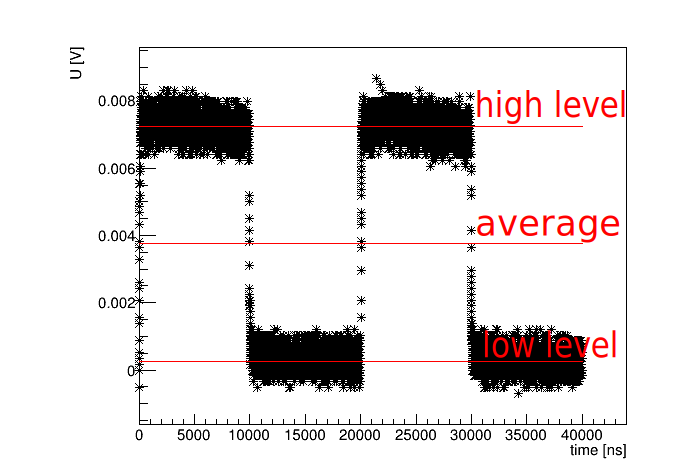
\includegraphics[scale=0.65]{./pictures/PMTPulse}
 \caption{Determining the basic pulse properties - average, low and high levels of signal.}
 \label{pulse}
\end{figure}

To determine the pulse height, we need to calculate the average value from all the samples at first. Then, we split the samples into two subgroups according to fact, whether they are higher or lower than the average. These subgroups are converted to histograms with fixed binning (around 5000 bins). These histograms are then fitted by gaussian. The means of these two fits determine two levels of the pulse - high ($U_\textrm{h}$) and low ($U_\textrm{l}$). The fig. \ref{pulse} shows the real pulse with levels determined by this method. The height of pulse is then simply calculated by substracting two levels: $U_\textrm{H} = U_\textrm{h} - U_\textrm{l}$.

\par
The properties the rising edge could be specified by two parameters, which we are able to extract from our data - time and the slope of the rising edge. We are able to calculate both of them if we identify the samples, which are taken at the time of the rising. These samples' values should be between 10 $\%$ and 90 $\%$ of the $U_{H}$. First, we need to detect the rising edge in waveform data sequence. However, the signal is very noisy and this could not be simply done by detecting the exceeding of the 10 $\%$ of the $U_{H}$ .To achieve that, we cycle through the waveform until we meet two conditions - the value is higher than average and the derivative is positive. Due to the noise, the derivative could not be calculated from two or three points, thus we use Savitzky–Golay polynom's derivative at chosen point: $y' = \frac{1}{12h}(y_{i-2} -8y_{i-1} + 8y_{i+1} - y_{i+2}) $. However we care only of positive/negative sign, so $\frac{1}{12h}$, where $h$ is the small step, is no use for us. When these two conditions are met at some point, the program cycles back from the point through the waveform until reaches $10\%$ level, and then beginning at the same point, which met the conditions, cycles up to reaching $90\%$ level. All the samples traversed by this way are considered as samples of the rising edge. The rising time is calculated simply by multipling the number of these samples by osciloscope's sample time (2 ns). The slope is calculated from linear fit of these samples (fig. \ref{linfit}).  


 \begin{figure}[H]
 \centering
 \includegraphics[scale=0.65]{./pictures/linFit}
 \caption{Linear fit of rising edge points (marked as green).}
 \label{linfit}
\end{figure}


\subsection{Results}

\section{UV LED diode aging}

%------------------------------------------------
\section{Optical feedback - potential fix}
% -----------------------------------------------
One way to handle the aging process of UV LED diodes is to monitor the power and according to the changes set the diode current. 


%------------------------------------------------

\section{Modified UV source for drone mounting}
% -----------------------------------------------



% -----------------------------------------------
% %%%%%%%%%%%%%%%%%%%%%%%% End of file %%%%%%%%%%%%%%%%%%%%%%%%

% -----------------------------------------------
% -----------------------------------------------
% Vlastní text práce (kapitoly práce)
% -----------------------------------------------

% -----------------------------------------------
\chapter{Calibration data analysis}
% -----------------------------------------------
In this section we present the analysis of calibration data, which we acquired by illuminating one FAST telescope (Argentina) by the older version of homogeneous UV LED source mounted into the IS. The older version of UV source was incapable of generating exact square pulse, and thus its output is deformed. However, the pulse's shape is stable and thus it was possible to use it for this experiment.   

\par
The main goal of this experiment is to obtain the relative responsivity ration constants for every of the four FASTs' PMTs (pixels) with respect to the pixel with greatest response for three positions of illumination - from left, right and bottom. Full specifications of the pixels numbering and positions could be seen on fig. \ref{PMT orientation}.

\begin{figure}[H]
 \centering
 \includegraphics[scale=0.35, angle = 0]{./pictures/orientation2.png}
 \caption{Orientation of FASTs' PMTs (pixels).}
 \label{PMT orientation}
 
\end{figure}

% -----------------------------------------------
\section{Calibration process}
% -----------------------------------------------
The UV source was mounted onto three positions and used as EULS to generate $8$ $\mu$s pulses. Two LED current levels were tested - $I_{d1} = 0.3$ mA and $I_{d2} = 0.8$ mA. These pulses trigger an event for the telescope - it acquires waveform data from every of the four PMTs. The PMTs' signal is converted into the number of photoelectrons registered in 20 ns. The example of detected 0.3 mA pulse from bottom position can be seen on fig (\ref{03pulse}). The 0.8 mA pulse is on fig. (\ref{08pulse}).

\begin{figure}[H]
 \centering
 \includegraphics[scale=0.3, angle = 0]{./pictures/CalibPulses.png}
 \caption{0.3 mA pulse registered by all pixels.}
 \label{03pulse}
 
\end{figure}

\begin{figure}[H]
 \centering
 \includegraphics[scale=0.3, angle = 0]{./pictures/CalibSaturated.png}
 \caption{0.8 mA pulse saturated two pixels.}
 \label{08pulse}
 
\end{figure}


The fig. \ref{08pulse} shows that the 0.8 mA pulse saturated the pixel 1 and 3 and thus it is not possible to use them in analysis. 


\par
The 0.3 mA pulses are suitable for our analysis. However, due to their deformation we are not able to use analogous analysis scheme as we did for calibration source testing. The best parameter describing the collection efficiency of the PMT is the pulse's integral. 

% -----------------------------------------------

\section{Analysis and results}
% -----------------------------------------------
The data includes 4 waveforms for every detected pulse event and consists around 800 pulse events (for every position). From these signal waveforms we calculate the pulse's integral and then use these signal integrals to construct histograms. These histograms are fitted by gaussian. This process is repeated for all the three positions.
\par
The fitted histograms can be seen on fig. \ref{leftCal} (left), \ref{rightCal} (right) and \ref{bottomCal} (bottom).
\begin{figure}[H]
 \centering
 \includegraphics[scale=0.32, angle = 0]{./pictures/left.png}
 \caption{Signal integral histograms with gaussian fits for left position.}
 \label{leftCal}
 
\end{figure}
\begin{figure}[H]
 \centering
 \includegraphics[scale=0.32, angle = 0]{./pictures/right.png}
 \caption{Signal integral histograms with gaussian fits for right position.}
 \label{rightCal}
 
\end{figure}
\begin{figure}[H]
 \centering
 \includegraphics[scale=0.32, angle = 0]{./pictures/bottom.png}
 \caption{Signal integral histograms with gaussian fits for bottom position.}
 \label{bottomCal}
 
\end{figure}


The main parameter for determining responsivity ration constants is the mean value of the signal integrals, which is extracted from the gaussian. The relative calibration constants are calculated as follows:

\begin{equation}
c_{\textrm{i}} = \frac{m_{\textrm{i}}}{m_{\textrm{ref}}}.
\end{equation}

Where $c_{\textrm{i}}$ is a relative responsivity ration constants for i-th pixel, $m_{\textrm{i}}$ - associated mean value and $m_{\textrm{ref}}$ - mean value of the reference pixel. As the reference pixel is chosen the one with the greatest responsivity. 
\par
The associated error is:
\begin{equation}
\mu(c_{\textrm{i}}) = c_{\textrm{i}} \sqrt{(\frac{\mu(m_{\textrm{i}})}{m_{\textrm{i}}})^2 + (\frac{\mu(m_{\textrm{ref}})}{m_{\textrm{ref}}})^2}.
\end{equation}

As the basic errors $\mu(m_{\textrm{ref}})$ and $\mu(m_{\textrm{i}})$ are taken only the errors from the gaussian fits. Other systematic uncertainties were not yet determined and are not considered in this thesis.
\par
The results calculated by these equations for every position can be seen in the following table.

\begin{table}[H]
\centering
\begin{tabular}{|c|c|c|c|}
\hline
   & right & left & bottom \\ \hline
$c_0$ & $0.2314 \pm 0.0002$    & $1$   				   & $0.1070 \pm 0.0002$     \\ \hline
$c_1$ & $0.1397 \pm 0.0002$    & $0.7485 \pm 0.0003$   & $0.8061 \pm 0.0003$      \\ \hline
$c_2$ & $0.9304 \pm 0.0004$    & $0.2138 \pm 0.0002$   & $0.1631 \pm 0.0002$      \\ \hline
$c_3$ & $1$    				   & $0.2462 \pm 0.0002$   & $1$      \\ \hline
\end{tabular}
\caption{Table of calculated relative responsivity ration constants.}
 \label{CalibConstTbl}
\end{table}


%------------------------------------------------

\section{Simulation compartment and discussion}

To discuss the relevancy of measured and calculated values, we compare them to their counterparts from optical simulations, which were designed by Mgr. Martin Vacula from SLO. These simulations consists of theoretical models of FAST's mirrors and pixels illuminated by EULS in same three positions as was defined before. These models includes inhomogeneity correction matrixes for every pixel.

\begin{table}[H]
\centering
\begin{tabular}{|c|c|c|c|}
\hline
   & right & left & bottom \\ \hline
$c_0$ & $0.48$    & $0.95$   & $0.44$     \\ \hline
$c_1$ & $0.41$    & $1$   	 & $0.98$      \\ \hline
$c_2$ & $1$    	  & $0.41$   & $0.46$      \\ \hline
$c_3$ & $0.95$    & $0.46$   & $1$      \\ \hline
\end{tabular}
\caption{Table of simulated relative responsivity ration constants by Mgr. Martin Vacula.}
 \label{CalibConstTblSim}
\end{table}

The compartment between the two tables (theoretical simulation - \ref{CalibConstTblSim} and the real measurement - \ref{CalibConstTbl}) shows that the two pixels, which are lesser illuminated at the specified position have lesser responsivity than they should have according to the simulations.

\par
These differences may be caused by uncertainties in the EULS positioning, its partial space inhomogeneity, mirror inhomogeneity, or some yet undiscovered phenomena.


% -----------------------------------------------



% -----------------------------------------------
% %%%%%%%%%%%%%%%%%%%%%%%% End of file %%%%%%%%%%%%%%%%%%%%%%%%

% -----------------------------------------------
% Závěr
% -----------------------------------------------
\chapter*{Conclusion}
\addcontentsline{toc}{chapter}{Conclusion}

We are completely f****d.

% -----------------------------------------------
% Literatura a prameny
% -----------------------------------------------
%\begin{thebibliography}{99}
\bibliographystyle{unsrt}
\nocite{*}
\bibliography{citations}
%\addcontentsline{toc}{chapter}{Literatura}
%\bibitem{gravitation} MISNER, Ch. W.; THORNE, K. S.; WHEELER, J. A. %\emph{Gravitation}. San Francisco: W. Freeman, 1973.
%\end{thebibliography}

\newpage
Preferované jsou citace podle norem ČSN ISO 690 a ISO 690-2, popř. styly APS (American Physical Society – u~prací zaměřených fyzikálně) nebo APA (American Psychological Association – u~prací zaměřených více didakticky a pedagogicky).
\end{document}
% Konec souboru %%%%%%%%%%%%%%%%%%%%%%%%%%%%%%%%%%%%%%%%%%%%%%%%%%%%%%%%%%%%
